\chapter{Background and Related work}

\section{Introduction Of Halide}
\quad\ \ Halide\cite{Halide1}\cite{Halide2} is a new programming language designed to make it easier to write high-performance image processing code on modern machines. Its current front end is embedded in C++. Compiler targets include x86/SSE, ARM v7/NEON, CUDA, Native Client, and OpenCL.
The following function defines and sets the schedule for a 3x3 box filter defined as a series of two 3x1 passes:

\lstset{language=C++} % Set your language (you can change the language for each code-block optionally)
\begin{lstlisting}[frame=single] % Start your code-block 

Func blur_3x3(Func input) {
  Func blur_x, blur_y;
  Var x, y, xi, yi;

  // The algorithm - no storage or order
  blur_x(x, y) = (input(x-1, y) + input(x, y) + 
  input(x+1, y))/3;
  blur_y(x, y) = (blur_x(x, y-1) + blur_x(x, y) +
  blur_x(x, y+1))/3;

  // The schedule - defines order, locality; implies storage
  blur_y.tile(x, y, xi, yi, 256, 32)
        .vectorize(xi, 8).parallel(y);
  blur_x.compute_at(blur_y, x).vectorize(x, 8);

  return blur_y;
}


\end{lstlisting}

Figure ~\ref{HalideCodegen} shows Halide codegen flow, after Halide programmers compile the source code the Halide compiler will compile it to llvm bitcode and transfer it to C/C++, OpenCL, OpenGL, renderscript and etc.With this feature,we compile our program to C++ and OpenCL, after the compilation we can use our framework to execute the Halide program of C++ and OpenCL synergistically.
\begin{figure}[H]
\centering
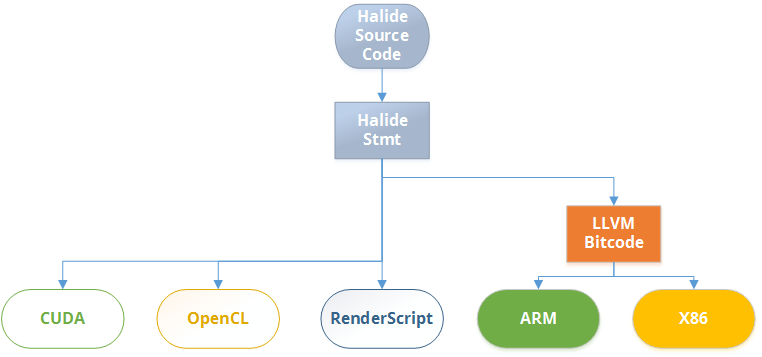
\includegraphics[width=10cm]{img/HalideCodegenFlow.png}
\caption{Halide Codgen Flow }
\label{HalideCodegen}
\end{figure}


\section{Introduction of OpenCL}
\quad\  \ Base on the respect of Halide, we will have a brief overview of the OpenCL programming standard. OpenCL is an open standard of computing for heterogeneous devices developed by Khronos Group. Vendors who support OpenCL for their devices ship OpenCL runtime software and compilation tools which facilitate development of OpenCL programs for their devices. Currently OpenCL is supported by most major CPU and GPU vendors including AMD, Intel, NVidia, ARM and Apple.OpenCL allows runtime software from different vendors to coexist and allows programs to utilize multiple platforms in the same program. 

OpenCL programs consist of the host program which runs on the CPU and coordinates activities with the runtime using API functions and kernel programs which run on the compute device.According to Halide,an OpenCL program will have 6 stages init\_kernels,  device\_malloc, copy\_to\_device, run,  copy\_to\_to\_host and device\_free."init\_kernels" includes clGetContextInfo, clGetDeviceInfo, clCreateProgramWithSource and clBuildProgram."device\_malloc" equals to "clCreateBuffer". "copy\_to\_device" is clEnqueueWriteBufferRect when choosing OpenCL as our backend."run" consists of clCreateKernel, clSetKernelArg, clEnqueueNDRangeKernel, clReleaseKernel and clFinish."copy\_to\_host" is clEnqueueReadBufferRect."device\_free" is clReleaseMemObject.

